\documentclass[11pt]{article}
\usepackage[utf8]{inputenc}
\usepackage{geometry}
\usepackage{graphicx}
\usepackage{hyperref}
\usepackage{amsmath}
\usepackage{amsfonts}
\usepackage{amssymb}
\usepackage{color}
\usepackage[capitalise,noabbrev]{cleveref}
\usepackage{caption}
\usepackage{subcaption}
\geometry{a4paper}

\title{MuesliSwap On-Chain Governance Platform}
\author{MuesliSwapTeam}
\date{\today}

\usepackage{biblatex}
\addbibresource{references.bib}


\begin{document}

\maketitle
% \newpage
% \tableofcontents
% \newpage

\section{Introduction}
\subsection{Background}
In the rapidly evolving world of blockchain technology, on-chain governance has emerged as a pivotal aspect for the sustainable and democratic management of decentralized protocols.
The intricate balance between decentralization, security, and efficiency poses unique challenges and opportunities.
This document delves into the cutting-edge realm of on-chain governance by presenting a comprehensive analysis and strategic implementation plan, focusing on the design and functionality of a treasury contract and an interface for protocol parameter updates on the Cardano Blockchain.

\subsection{Purpose of the Document}
The primary objective of this document is to serve as a detailed guide for the development, analysis, and integration of advanced governance mechanisms within blockchain protocols.
It aims to provide a robust framework for designing a treasury contract, an interface for updating protocol parameters, and a comparative analysis of existing on-chain governance solutions.
This document is intended for developers, stakeholders, and decision-makers involved in blockchain governance and development.

\subsection{Scope}
The scope of this document encompasses three main areas:
Firstly, it provides a detailed design and functional specification for a treasury contract and a protocol parameter update interface, ensuring these components align with the overarching goals of security, transparency, and user accessibility.
Secondly, it presents a comparative analysis of existing on-chain governance models, highlighting their strengths, weaknesses, and applicability in various contexts.
Lastly, it outlines a comprehensive integration plan for embedding these governance components into an existing off-chain voting platform, detailing the technical, procedural, and risk management aspects of such an integration.
This holistic approach ensures a thorough understanding and effective implementation of on-chain governance solutions.


\section{Detailed Design and Functional Specifications}

This section outlines the desired capabilities and functionality of the MuesliSwap On-Chain governance platform.

\subsection{Overview of the Platform}
The platform consists of a set of smart contracts that allow control over funds and on-chain parameters
of the MuesliSwap development treasury and decentralized exchange.
Moreover it provides a user friendly interface for the community to propose and vote on proposals.
It complements the existing governance forum, which is available to facilitate discussion on MuesliSwap governance,
as well as the existing off-chain governance platform that allows secure, private and scalable voting.

\subsubsection{Objectives}
The governance platform is built to allow holders of the MuesliSwap MILK token to participate in
decisions that affect the MuesliSwap protocol proportional to their stake in the project in form of holdings.
It should further allow any holder of the MILK token to propose changes to the protocol and
vote on proposals that are submitted by other users.
The results of proposals should be binding and enforceable by the smart contracts and will be documented
on-chain through the nature of the platform.

\subsubsection{Design Principles}

The platform will by design represent most interactions by submitting transactions to the Cardano blockchain.
These will be transparently visible to all users and verifiable by anyone.
We note that this may incur cost for users, which is outlined in recent studies as a major drawback of on-chain governance \cite{feichtinger2023hidden}.

However, due to the integration with the off-chain governance platform, users will be able to vote on-chain
only for situations where the benefit of on-chain governance (e.g. transparency, enforceability) justifies the cost of the process.

The platform is designed such that the governance process can not be controlled by a single entity.

Another key factor is modularity in the design.
The platform will mainly take care of tallying votes.
Contracts that are affected by the voting process will be responsible for handling the effects of the voting process themselves.
This includes i.e. the MuesliSwap Pools contract, which needs to be upgraded such that it can process the outcome of votes.
The treasury is provided in the development of this project as a reference implementation of such a contract.

Meanwhile, the contract supports the possibility of an upgrade.
This is to ensure that the contract can be upgraded in case of a bug or security vulnerability or simply to support
relevant features.
Rather than forcing every consumer to upgrade the consumed contract,
the contract will allow moving the governance thread to a new contract version.
The alternative would be to allow consumers to upgrade the Tally contract which they track -
which implies that for every upgrade of the Tally contract, every consumer would have to be upgraded as well.
This would be a major burden for consumers of the contract and can lead to security issues due to pending upgrades.

To avoid double voting, it is necessary to lock governance tokens during the voting process.
The protocol is designed to minimize the time that tokens are locked and to reduce the cost of participation.
In subsequent extensions, we will explore the possibility of allowing users to delegate their voting power to other users,
use staked tokens for participation in the governance process, and other mechanisms to reduce the cost of participation.

\subsubsection{Architecture}
\label{sec:architecture}

The protocol consists of a set of smart contracts that are deployed on the Cardano blockchain.
The main component is the \emph{Tally} contract, which is responsible for the overall governance process.
It is used to track submitted proposals by users and tally voting results.
Users join the governance process by locking funds into the \emph{Staking} contract (see \cref{fig:utxo-flow-gov-stake-init}).
The Staking contract tracks the tallies that the funds are participating in and ensures that
the voting power of the funds is locked for the duration of the voting process where the funds are participating.

Users can consume the current state of the proposal and their staked tokens to add their vote to the tally,
in the process updating the staking state such that its funds are locked until after the voting period has ended.
Should they decide to withdraw their vote before the end of the voting period, they can do so by consuming the
state of the propsal and the staking state.
This process is depicted in \cref{fig:utxo-flow-vote-complete}.

\begin{figure}
    \centering
    \begin{subfigure}[b]{0.5\textwidth}
        \centering
        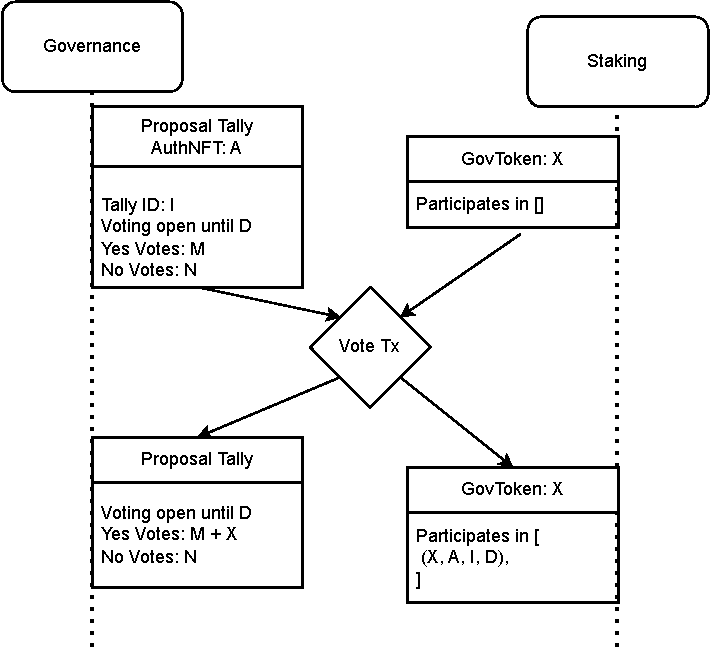
\includegraphics[width=\textwidth]{figures/gov-vote.pdf}
        \caption{Voting consumes the current state of the proposal and informs the staking contract that funds are participating in a tally.}
        \label{fig:utxo-flow-vote}
    \end{subfigure}
    \hfill
    \begin{subfigure}[b]{0.35\textwidth}
        \centering
        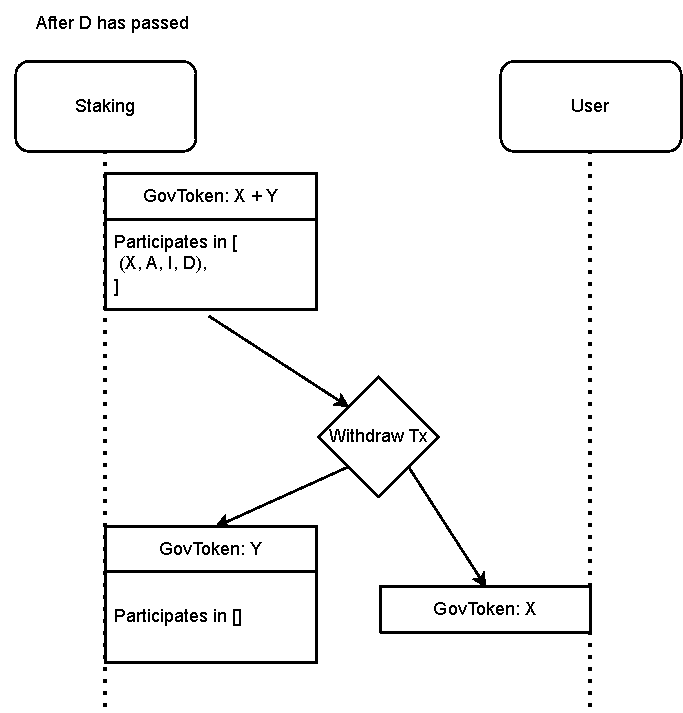
\includegraphics[width=\textwidth]{figures/gov-withdraw-after.pdf}
        \caption{After the voting period has ended, the user can withdraw their locked funds.}
        \label{fig:utxo-flow-withdraw}
    \end{subfigure}
    \hfill
    \vspace{1em}
    \begin{subfigure}[b]{0.5\textwidth}
        \centering
        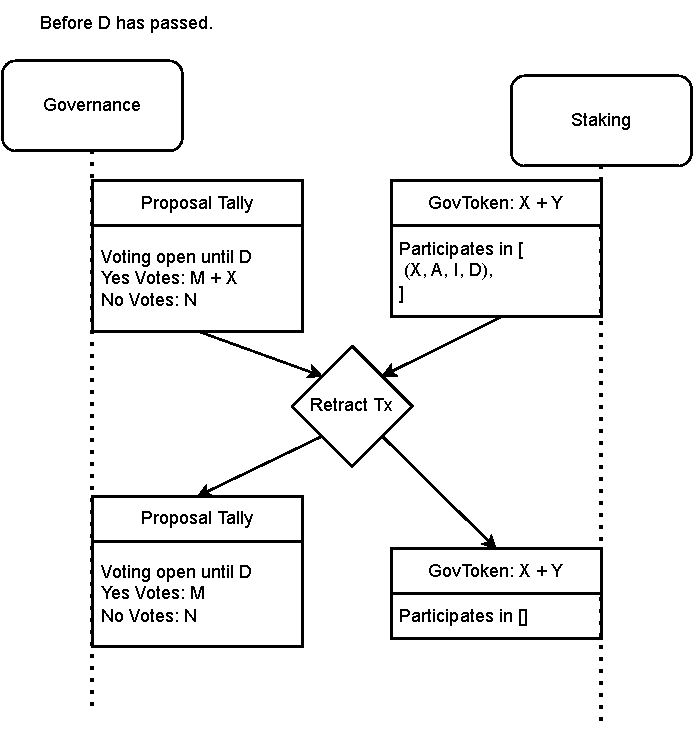
\includegraphics[width=\textwidth]{figures/gov-withdraw-before.pdf}
        \caption{The user can retract a vote by consuming the current state of the proposal and the staking status.}
        \label{fig:utxo-flow-retract}
    \end{subfigure}
    \caption{Example UTxO flow for a vote.}
    \label{fig:utxo-flow-vote-complete}
\end{figure}

Moreover there is one \emph{Treasury} contract for managing the funds of the MuesliSwap development treasury.
It processes the outcome of the voting process and executes the result of the vote by distributing the funds correspondingly.
The handling of protocol parameter updates is left to the specific parameterizable protocol components,
such as the MuesliSwap \emph{Pools} contract.

\subsection{Protocol Parameter Update Interface}

The result of the voting process will remain as an immutable tally result in the Tally contract
indefinitely.
Thus it can be consumed by the protocol components as a reference UTxO to update their internal state accordingly.
An example of the parameter updates that are possible through the Tally contract is the changing of pool swap fees
or changing its stake key.
An example UTxO flow is depicted in \cref{fig:utxo-flow-params}.

\begin{figure}
    \centering
    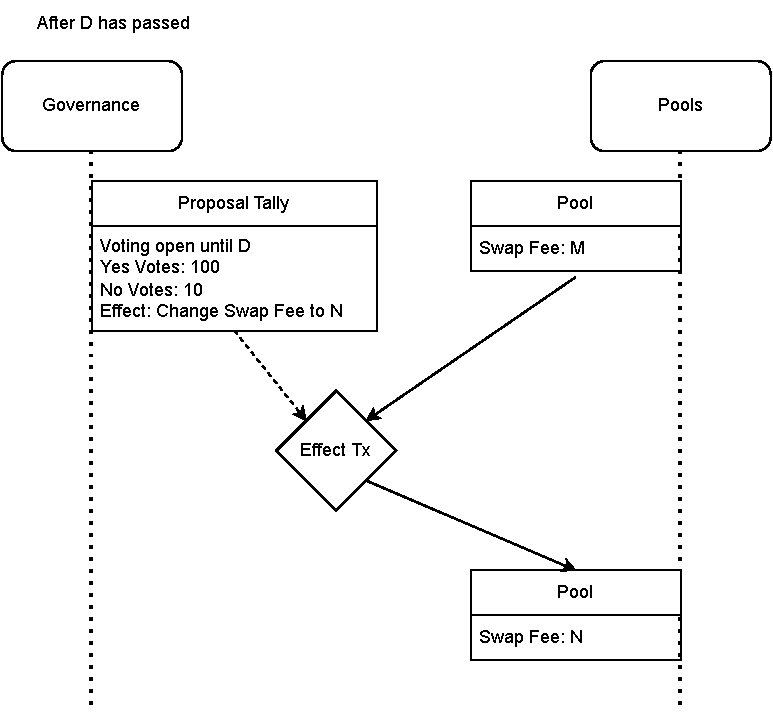
\includegraphics[width=0.5\textwidth]{figures/pool-param-update.pdf}
    \caption{Example UTxO flow for a parameter update}
    \label{fig:utxo-flow-params}
\end{figure}

\subsection{Treasury Distribution Interface}

The Treasury contract will be responsible for managing the funds of the MuesliSwap development treasury.
For this, the result of the voting process will be consumed by the Treasury contract and the funds will be distributed accordingly.
To allow parallel and contention-free deposits into the treasury, the treasury is split in two parts:
The \emph{Treasurer} contract and the \emph{Value Store} contract.

Deposits into the Value Store can be performed by any user.
Deposits are accompanied by a datum that specifies the treasurer that is responsible for spending the funds.

The Treasurer contract keeps track of which tally results have already been processed to prevent distributing funds multiple times.
In a distribution transaction, it sums the funds spent from the Value Store and ensures that only what can be distributed according to the tally result is spent.
The remaining funds are returned to the Value Store.
The resulting UTxO flow is depicted in \cref{fig:utxo-flow-treasury}.

\begin{figure}
    \centering
    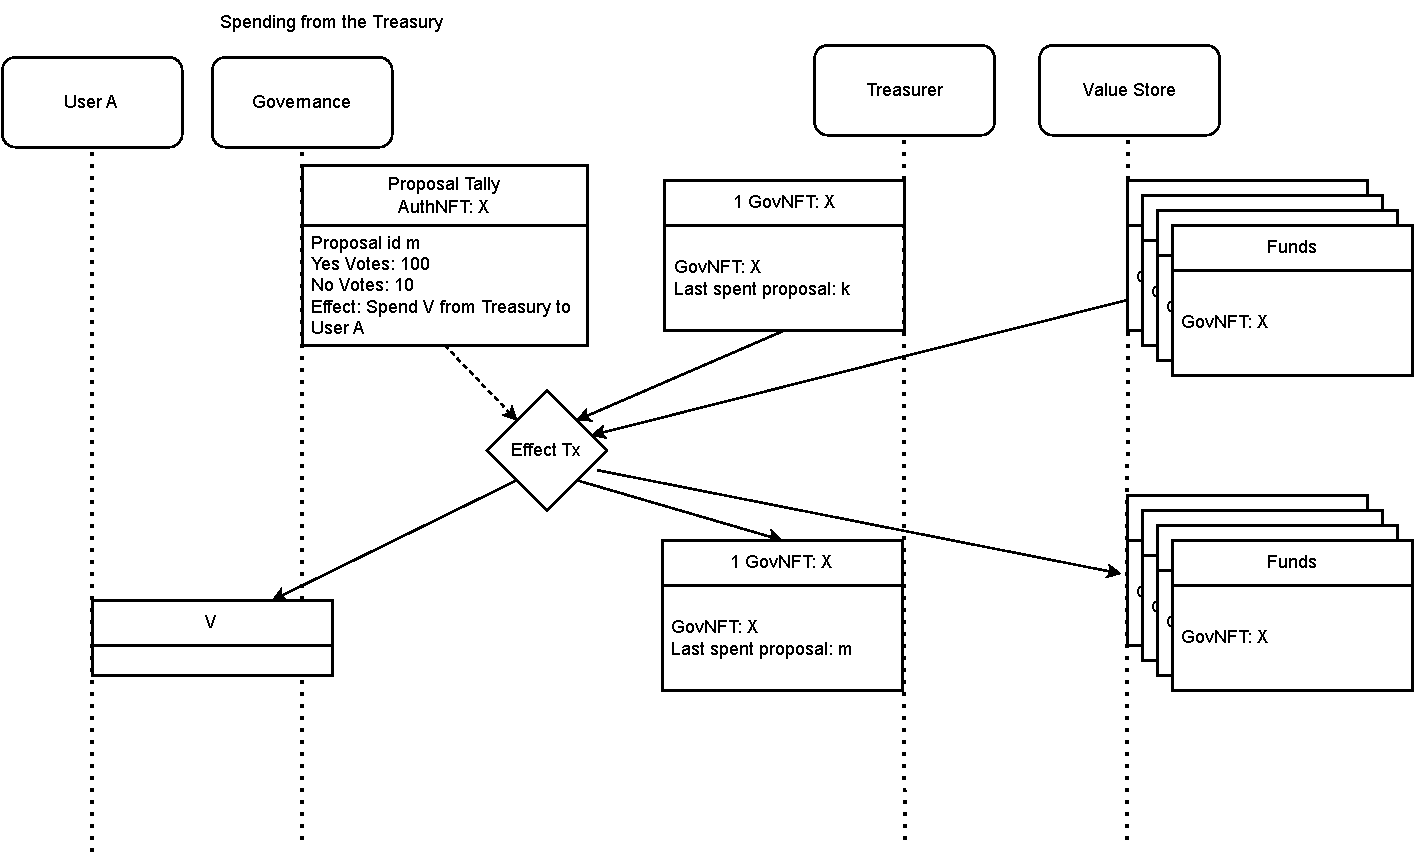
\includegraphics[width=0.5\textwidth]{figures/spend-from-treasury.pdf}
    \caption{Example UTxO flow for a treasury spending}
    \label{fig:utxo-flow-treasury}
\end{figure}

\subsubsection{Functional Requirements}

The platform needs to allow every token holder to participate in the governance process by submitting or voting on proposals.
To this end, both accessible user-interfaces as well as manual interaction with the contracts must be possible.
The platform needs to ensure that operability is not centralized, i.e. that no single entity can control the outcome or block the progressing of the voting process.

\subsubsection{User Interface Design}
The user interface will be oriented along the existing off-chain governance platform.
It is crucial to ensure that the user interface is intuitive and easy to use and displays all relevant information
of the on-chain proposals and votes clearly and concisely.

\subsubsection{Security Considerations}

To avoid spam, the platform will require a minimum amount of tokens to be locked in order to submit a proposal.
In case the proposal passes, the locked tokens will be returned to the submitter.
In case the proposal fails, the locked tokens will be distributed to the voters or the treasury.
Allowing distribution to voters creates a natural incentive to participate in the voting process, even if it is expected that the proposal will fail.
Distribution to the treasury increases the value of the treasury and thus the value of the protocol.
A split between these choices is also a reasonable option.

It is crucial to ensure that voting results can only be effectful once for each component that they influence.
Otherwise it may be possible to withdraw funds multiple times from the treasury or to change a parameter to an outdated value after a new proposal has been passed.
Therefore every proposal will be assigned a monotonously increasing proposal ID.
Protocol components must then ensure that they only allow consumption of a strictly increasing proposal ID.

Moreover it is important to ensure that controlled funds can only be counted once for each proposal.
For this purpose the staking contract is used that keeps track of all the proposals that the locked funds are participating in.
The staking contract further needs to ensure that no third party can create a staking position on behalf of another user.
This would allow retracting votes for other users, which is not desired.

\section{Comparative Analysis of Existing Governance Solutions}

In this section we explore the current state of On-Chain and Off-Chain Governance solutions on Cardano.
Further we explore design choices in other blockchain ecosystems.

\subsection{Methodology}
This subsection delineates the methodology employed in the comparative analysis of existing on-chain governance solutions.
The primary goal of this analysis is to critically assess and compare various governance models,
highlighting their unique features, strengths, and limitations in the context of blockchain technology and decentralized decision-making processes.

\subsubsection{Selection Criteria for Governance Models}

First of all, we try to collect all governance models currently deployed or under development on the Cardano blockchain.
In addition, we explore governance models that are deployed on other blockchains based on their prevalence in the industry, innovativeness, impact on user engagement, and scalability.

\subsubsection{Data Collection and Sources}
Data and information regarding each governance model are collected from a variety of sources, including academic journals, press releases, reports and whitepapers.
This comprehensive approach ensures a well-rounded understanding of each model and its real-world implications.

\subsubsection{Evaluation Metrics}
The comparative analysis employs a set of predefined metrics to evaluate each governance model.
These metrics encompass:

\begin{itemize}
    \item \textbf{Efficiency:} Assessing the speed and resource utilization in decision-making processes.
    \item \textbf{Security:} Evaluating the robustness of each model against common threats and vulnerabilities.
    \item \textbf{Decentralization:} Measuring the degree of power distribution among participants.
    \item \textbf{User Incentivization:} Analyzing how each model encourages and facilitates active participation from its stakeholders.
\end{itemize}

\subsubsection{Analytical Approach}
The analysis is conducted through a multi-dimensional approach, considering both qualitative and quantitative aspects of each model. Qualitative analysis provides insights into the governance structure, user experience, and potential socio-economic impacts. Quantitative analysis, on the other hand, involves statistical evaluation of performance metrics and user engagement data.

\subsubsection{Comparative Framework}
A structured comparative framework is employed to systematically evaluate each model against the set metrics. This framework aids in highlighting the contrasts and similarities among the various governance models, providing a clear and concise comparative overview.

\subsubsection{Limitations and Assumptions}
The methodology acknowledges certain limitations and assumptions. Limitations may arise from the availability and recency of data, while assumptions are made regarding the general applicability of each model in different blockchain ecosystems. These factors are taken into account to ensure a balanced and fair analysis.

The outcome of this methodology is expected to provide valuable insights into the effectiveness and applicability of different on-chain governance models, guiding future developments and decision-making processes in the realm of blockchain governance.

\subsection{Governance Models on Cardano}

We explore a comprehensive set of governance models, including both on-chain and off-chain solutions
that are currently in use on the Cardano Blockchain.

\subsubsection{MuesliSwap Off-Chain Governance}

The MuesliSwap Off-Chain Governance platform is a decentralized voting platform that allows users to vote on proposals regarding the MuesliSwap protocol \cite{muesliswap-offchain}.
It is built on top of the peer-reviewed Helios protocol \cite{DBLP:conf/uss/Adida08}.
This platform allows for secure, private, and scalable voting, while ensuring that the results of the vote are publicly verifiable.
At the same time, the design of the platform ensures that no fees are incurred for neither the platform operators nor the voters.

However, due to the nature of being entirely off-chain the protocol does not allow for enforceable on-chain effects of the voting result.
It is therefore not further analyzed in this document.

\begin{itemize}
    \item \textbf{Efficiency:} High. As an off-chain solution, the method can scale well.
    \item \textbf{Security:} High. The protocol is based on the peer-reviewed Helios protocol that ensures verifiability and privacy.
    \item \textbf{Decentralization:} Low. The MuesliSwapTeam is hosting the results on a server, which may be subject to failure. A selected set of administrators is able to create and tally votes. Results are not enforceable on-chain.
    \item \textbf{User Incentivization:} Medium. While not incurring any additional costs for participants, there is also no direct incentive for users to participate in the voting process.
\end{itemize}

\subsubsection{SundaeSwap On-Chain Governance}

SundaeSwap is a decentralized exchange built on the Cardano blockchain
and has recently also launched their own ``on-chain governance''\cite{Labs-2023}.
It works in the same fashion as the MuesliSwap Off-Chain Governance,
however it publishes commitment to user votes on the Cardano blockchain.

Users can thus verify that their vote has been taken into account by checking the produced on-chain commitment.
This increases the immutability of the voting process and allows for a more transparent process,
at the cost of increased transaction fees for the protocol operators.

Since this governance model is very similar to the MuesliSwap Off-Chain Governance and does not allow
any on-chain effects of the voting process, it will not be analyzed in detail in this document.

\begin{itemize}
    \item \textbf{Efficiency:} High. As a mainly off-chain batching solution, the method can scale well.
    \item \textbf{Security:} Unclear. The implementation is not yet available and the security of the protocol is not clear from the documentation.
    \item \textbf{Decentralization:} Low. SundaeSwapLabs is required to continue running a server to publish results on-chain, which may be subject to failure. A selected set of administrators is able to create and tally votes. Results are not enforceable on-chain.
    \item \textbf{User Incentivization:} Medium. While not incurring any additional costs, there is also no direct incentive for users to participate in the voting process.
\end{itemize}

\subsection{Wingriders On-Chain Governance}

Wingriders is a decentralized exchange built on the Cardano blockchain.
They have launched their own on-chain governance platform in October 2022 \cite{wingriders-medium}.
There is not much detail on its operation available online, but a published auditing tools for votes
indicates that the voting process simply consists of submitting a transaction to the Cardano blockchain with metadata indicating their preference.
This implies zero privacy for participants, as their voting preference is directly linked to their wallet address and publicly accessible,
however also ensures immutability and transparency.
The protocol operators tally the results by taking a snapshot of the voter wallets and their respective voting power at the end of the voting period. \cite{wingriders-github}
The only way to ensure correct tallying is by rerunning the whole tallying procedure.

The Wingriders protocol allows any user to submit proposals,
however requires a minimum amount of tokens to be locked in order to submit a proposal.
This serves as a spam protection mechanism and ensures that only serious proposals are submitted.

This governance model is rather centralized, as the voting process is controlled by the protocol operators.
It does not also not allow for any enforceable on-chain effects of the voting process,
since metadate is invisible to Cardano Smart Contracts.
It is therefore not further analyzed in this document.

\begin{itemize}
    \item \textbf{Efficiency:} High. Users submit Metadata transactions to the Cardano blockchain. This scales proportional with overall throughput of the Blockchain.
    \item \textbf{Security:} High. The protocol uses the Cardano blockchain to ensure verifiability and immutability.
    \item \textbf{Decentralization:} Medium. Results have to be tallied by the protocol operators and results are not enforceable on-chain.
    \item \textbf{User Incentivization:} Low. Participation incurs cost and there is no direct incentive for users to participate in the voting process.
\end{itemize}

\subsubsection{Agora}
LiqwidDAO's governance system is built upon an open-source governance framework called Agora\cite{liqwidagora}, developed by Liqwid Labs.

LiqwidDAO's Agora consists of interconnected smart contracts that together create a governance framework.
In this system, users can participate by staking their LQ tokens.
This staking process grants them the ability to initiate and cast votes on various proposals.
The influence of a user's vote is directly proportional to the quantity of LQ tokens they have staked.
Each stake is associated with the user's public key, ensuring that proposing an idea or voting on one necessitates verifying one's identity by signing the transaction with the corresponding key.

Further, the whole system is built on top of the Cardano blockchain, which ensures that all transactions are immutable and transparent.
Votes are not private.
Every vote has to consume the current state of the proposal, which is a UTxO that is updated by the Agora contract.
This means that the scalability of the system is limited by the fact that all votes have to be submitted in serial order, as they consume the current state of the proposal.

\begin{itemize}
    \item \textbf{Efficiency:} Low. The protocol involves submitting votes and updates to the governance progress in series and thus does not scale well.
    \item \textbf{Security:} High. The protocol uses the Cardano blockchain to ensure verifiability and immutability.
    \item \textbf{Decentralization:} High. The protocol allows for on-chain enforceability of the voting results. The voting process is not controlled by a single entity.
    \item \textbf{User Incentivization:} Low. Participation incurs cost and there is no direct incentive for users to participate in the voting process.
\end{itemize}

\subsubsection{Clarity DAO}

Clarity DAO is a project focusing on providing DAO infrastructure to projects on Cardano \cite{panchot2023clarity}.
The Clarity Protocol is built on top of Agora and does hence not require an additional investigation regarding protocol performance.


\subsubsection{Indigo DAO}

The Indigo DAO source code can be found on GitHub\footnote{\url{https://github.com/IndigoProtocol/indigo-smart-contracts/tree/main/src/Indigo/Contracts/Governance}}.
According to the developers it supports sharding of vote tallies and compositional upgrades using minting policy ids to control the execution of governance results.
It is not documented in detail however and further covered in this document.

\subsubsection{Distributed Representation by Logical Mechanism}

There is another GitHub repository featuring a DAO implementation for Cardano\footnote{\url{https://github.com/logicalmechanism/distributed_representation}}.
However to our knowledge, it is not yet deployed on the Cardano blockchain and not well documented.

\subsection{Governance Models on other Platforms}

In addition, we explore design choices of governance models that are deployed on other blockchains.
They are not explored in detail, but provide valuable insights into the design space of on-chain governance.

\subsubsection{Aragon Network}

Aragon is an advanced DAO building infrastructure built on Ethereum \cite{aragon}.
It is a suite of smart contracts and tools that enable the creation of DAOs with advanced features such as token issuance, voting, and fundraising.
Aragon's governance model is based on the concept of liquid democracy, where users can delegate their voting power to other users.
This allows for a more efficient and flexible voting process, as users can choose to vote directly or delegate their voting power to a trusted party.

\subsubsection{Tally / OpenZeppelin Governor}

Tally is a voting platform built on top of the OpenZeppelin Governor contract \cite{Tally, OpenZeppelin}.
The OpenZeppelin Governor contract is a central piece of software that controls the voting process, keeps tallys and also enforces outcomes of votes.
Among the feature set already delivered with the Governor contract is ``disbursing funds from a treasury, adjusting parameters of a DeFi protocol, altering permissions of sub-DAOs, minting NFTs, or even modifying the rules of the Governor contract itself''.
The contracts are entirely on-chain, therefore also require transactions for interaction.

\subsection{Best Practices and Lessons Learned}

From the analysed platforms, we learn that on-chain governance is a powerful tool to increase transparency and immutability of the governance process.
However, one must carefully consider the choice of parameters and security guards like spam protection.

Moreover, all contract governed protocols require the locking of tokens during the voting process to avoid double voting.
Other approaches make use of snapshots, which are currently infeasible to perform on-chain on Cardano
without a significant form of centralization (in the form of an oracle).

We also discover that most on-chain governance platforms do not allow for enforceable on-chain effects of the voting process,
which is a major drawback of these platforms.
At the same time, we acknowledge that the scope of potentially interesting effects is massive.
Therefore, we propose a modular approach to on-chain governance, where the governance platform is responsible for tallying votes and
custom implementations of protocol components are responsible for handling the effects of the voting process.

Moreover we find that on-chain governance systems usually allow for self-upgrade of the governance contract,
and will follow this path.
Note that on top of the governance contract,
consuming protocols can implement their own upgrade mechanism.

Due to the lack of enforceable on-chain governance contracts, we conclude that the MuesliSwap On-Chain Governance platform will be a valuable addition to the MuesliSwap ecosystem and the Cardano Ecosystem as a whole.

\section{Integration Plan for New Governance Components}
\subsection{Overview of the Off-Chain Voting Platform}

The current governance platform on MuesliSwap allows users to submit and vote on proposals tracked in an efficient and secure off-chain voting platform.
The platform can be accessed through the internet\footnote{The governance platform can be accessed at \url{https://vote.muesliswap.com}} and users can connect
their Web3 wallets to the platform to participate in the voting process.
Votes are tallied off-chain and cryptographically signed by the participants, then weighted by the amount of tokens that the participants hold.

The governance platform is built on top of a modified helios server \cite{DBLP:conf/uss/Adida08}.
This introduces additional complexity when trying to integrate a conceptually different on-chain governance platform.

\subsection{Integration Strategy}

Since the current governance platform is conceptually very different and re-using the existing platform is not feasible,
we propose to integrate the new on-chain governance platform in a separate process.
This involves designing a new user interface for the on-chain governance platform,
as well as a new backend that interacts with the Cardano blockchain.
The existing governance platform will continue to operate as usual and will be used to discuss proposals and to vote on proposals that do not require on-chain effects.
Since the new user interface will be built from scratch, it will be possible to integrate the old off-chain governance platform into the existing governance platform natively in the future.
Until then, the off-chain platform can be integrated visually by linking to the existing platform from the new user interface.

\subsubsection{Technical Requirements}

The new on-chain governance platform will be built on top of the Plutus smart contract platform.
To have proper access to the Cardano blockchain, the new platform will require a dedicated backend.
This backend connects to the Cardano blockchain through a Cardano node and processes transactions
to pre-process information about votes and proposals.

The backend should support the following features:
\begin{itemize}
    \item \textbf{Proposal Overview:} The backend should provide the list of valid user submitted proposals.
    \item \textbf{Proposal Details:} The backend should provide the details of a specific proposal, including the current tally state, deadlines and votes by other users.
    \item \textbf{Staking Status:} The backend should provide the staking status of a user, i.e. the weight of user votes and which proposals the user is participating in.
\end{itemize}

The user interface or frontend will connect to the backend and display the information to the user.
Further it will allow the user to submit new proposals, vote on proposals and withdraw votes.
For scalability and security, transactions will be built on the client side through the frontend.

\subsubsection{Modification of Existing Components}

The existing governance platform will not be modified in the process.
However, the new governance platform will allow integration of the existing platform in the future.
This implies that there will be a transition away from the existing platform in the future.


\subsubsection{Adding New Components}

The new governance platform will be built from scratch.
It will consist of a backend that connects to the Cardano blockchain and a frontend that connects to the backend.
These are entirely new components.

\subsubsection{Implementation Steps}

The implementation of the new governance platform will be done iteratively and accompany the development of the underlying protocol.
A development of a backend in lockstep with the contract development already helps to ensure that the contracts are usable and that the backend can be tested.
The frontend can assist in the development of the backend by providing a user interface to test the backend.
Moreover the ability to submit transactions through the frontend will allow testing of the contracts in a realistic environment.

Overall, the smart contract basics will be developed first.
This includes the Tally contract, the staking contract and the treasury contract.
The backend will then be developed to interact with the contracts.
Finally, the frontend will be developed to interact with the backend.
While there is this fundamental dependency between the components, the development of the components can be done in parallel and iteratively refined as the development progresses.


\section{Technical Details}

This sections outlines concrete elements of the final implementation of the MuesliSwap On-Chain Tally platform,
as well as outlining the UTxO flow for a few more activities.

\subsection{Main Components}

The implementation of the governance platform is designed with the following components.
\begin{itemize}
    \item \textbf{GovNFT:} A smart contract that allows minting of one-shot NFTs that have unique names ensured by hashing their input UTxO which is spent in the process.
    \item \textbf{AuthNFT:} A smart contract that allows minting of NFTs with the same name as a GovNFT, when a GovNFT is spent. This is used to authenticate tally results and should be tracked by consumers.
    \item \textbf{GovState:} The governance state contract tracks an initialized DAO configuration together with a unique, one-shot minted NFT, the GovNFT.
    \item \textbf{Tally:} The Tally contract tracks the current state of a proposal and allows for tallying votes.
    \item \textbf{Staking:} The staking contract locks funds for the duration of the voting process.
    \item \textbf{Treasury:} A treasury contract, which is a consumer of proposals of the Tally contract and distributes funds according to the outcome of the voting process.
    \item \textbf{VaultFT:} A fungible token contract, used to track funds locked in the MuesliSwap Vault and to allow delegating those funds to votes via the staking contract.
\end{itemize}

Note that consumers of the Tally contract can be any contract that is parameterizable by the voting process.
The important part is that the contract ensures that tally results are only valid if the AuthNFT is present and matches the expectation.
While the GovNFT is the token of actual interest, it can not be replicated and hence can not accompany the tally result, which will be consumed by the consuming contract.
Moreover, consumers need to ensure that a tally result can only be applied once by tracking the last applied proposal ID.

To set up a DAO structure, a governance thread has to be initiated by minting a GovNFT.
It is sent to the GovState contract, together with a datum that describes the the initial DAO configuration.
The process is depicted in \cref{fig:utxo-flow-gov-thread-init}.

The thread has to be consumed to create a vote on the Tally Contract, which is a proposal that can be voted on.
The process for tally initiation is depicted in \cref{fig:utxo-flow-vote-init}.
The general idea of how to update a tally result is presented in \cref{sec:architecture}.

By consuming the thread and governance NFT, the GovState contract can control whether an AuthNFT can be minted which needs to accompany the tally result. 
This ensures that it is enough for consumers to track the immutable AuthNFT to verify the final tally result.
Tracking the governance thread address or tally address may be insufficient,
as these contracts may be upgraded, as depicted in \cref{fig:utxo-flow-gov-thread-upgrade}.
An upgrade may change the GovState contract, parameters in the thread i.e. the DAO configuration or both.
The independence of AuthNFT/GovNFT and GovState and Tally ensures that the DAO can be upgraded without requiring consumers to upgrade their contracts,
and remains flexible and resilient for the future.

\begin{figure}
    \centering
    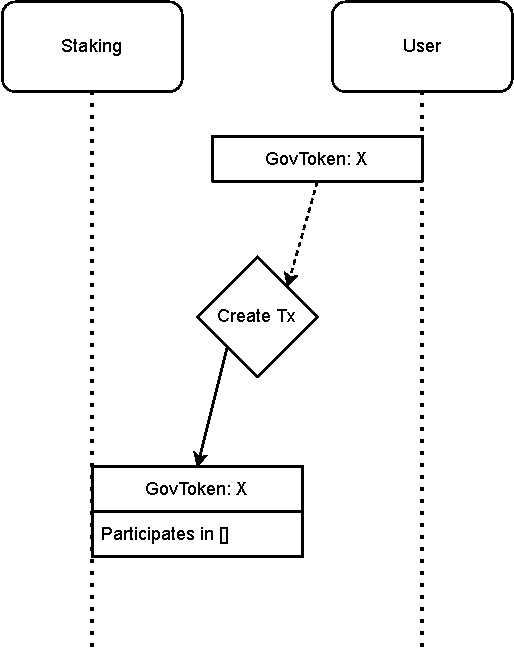
\includegraphics[width=0.35\textwidth]{figures/gov-init-stake.pdf}
    \caption{Example UTxO flow for the initialization of a staked position.}
    \label{fig:utxo-flow-gov-stake-init}
\end{figure}

\begin{figure}
    \centering
    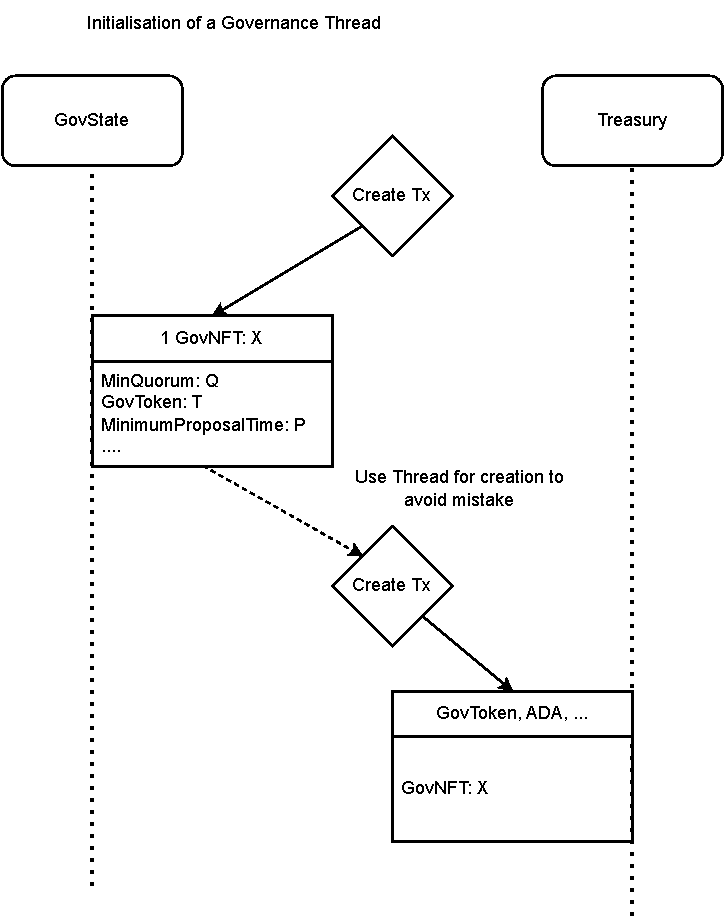
\includegraphics[width=0.35\textwidth]{figures/init-gov-thread.pdf}
    \caption{Example UTxO flow for the creation of a governance thread.}
    \label{fig:utxo-flow-gov-thread-init}
\end{figure}

\begin{figure}
    \centering
    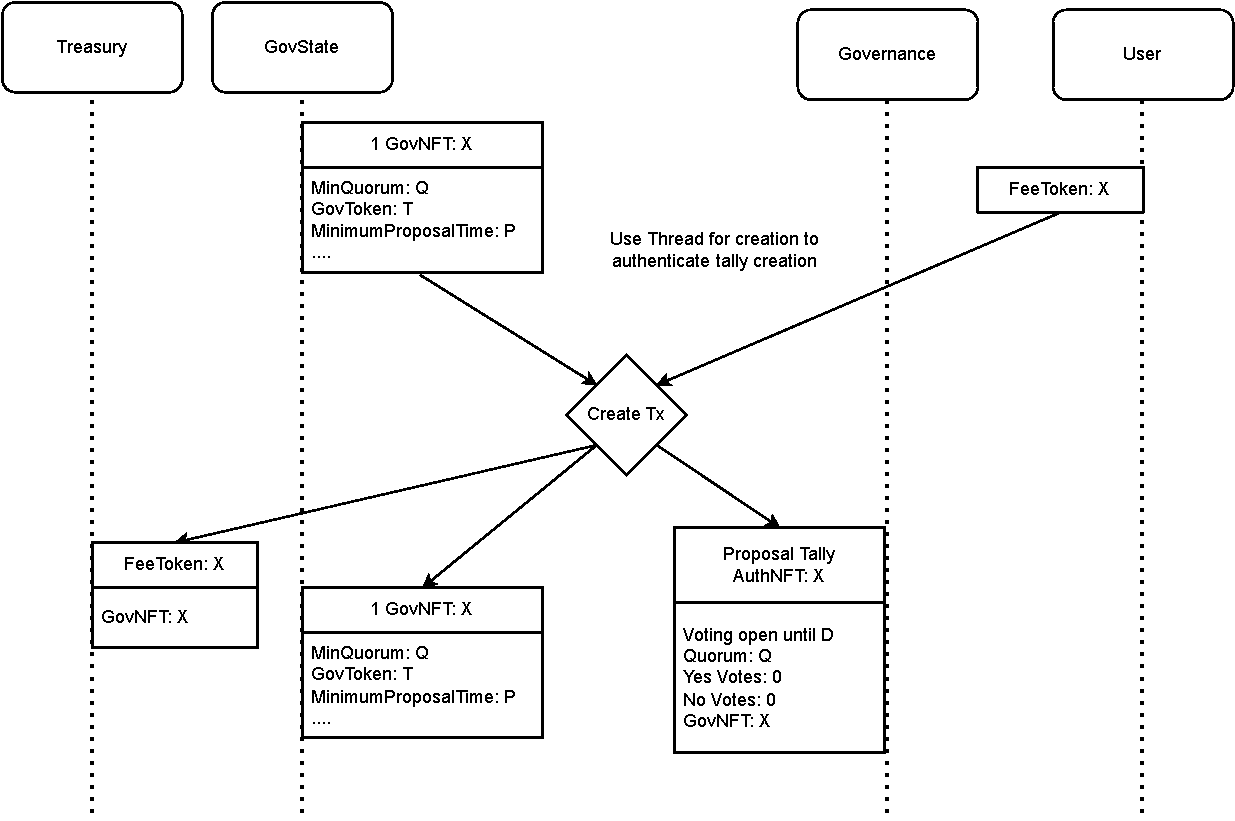
\includegraphics[width=0.35\textwidth]{figures/init-vote.pdf}
    \caption{Example UTxO flow for the creation of a governance vote.}
    \label{fig:utxo-flow-vote-init}
\end{figure}

\begin{figure}
    \centering
    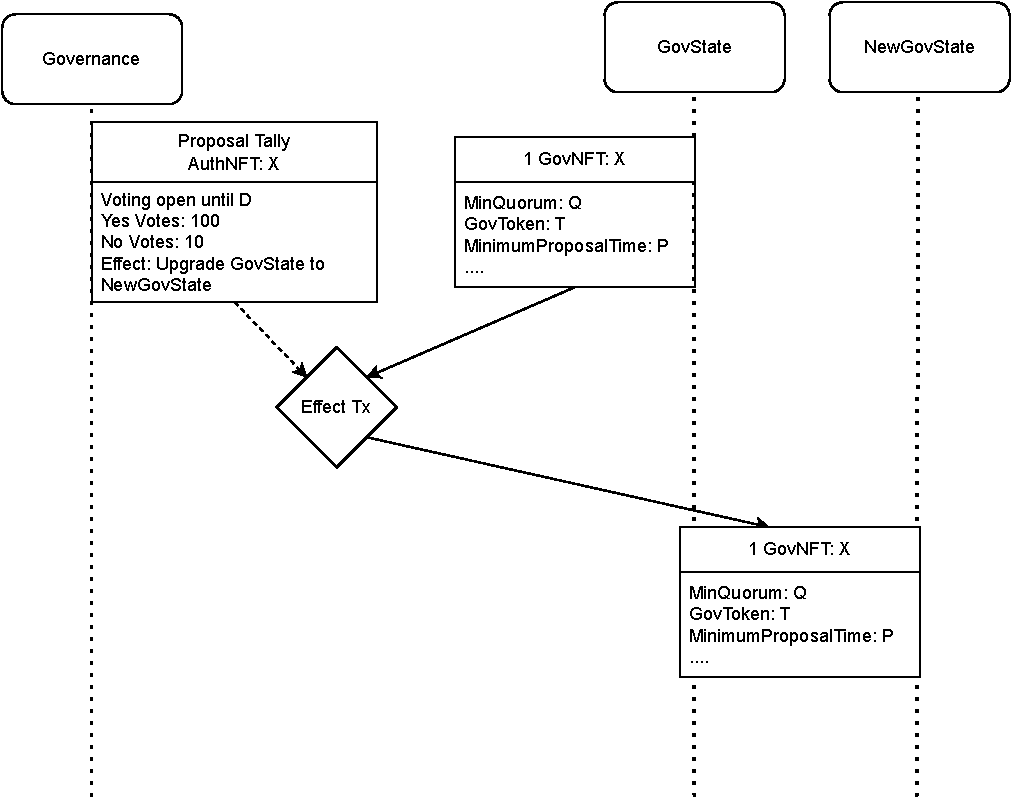
\includegraphics[width=0.35\textwidth]{figures/upgrade-gov-thread.pdf}
    \caption{Example UTxO flow for upgrading the governance thread.}
    \label{fig:utxo-flow-gov-thread-upgrade}
\end{figure}


\subsection{What precisely does every contract control?}

In order to check the validity of this modular contract, we outline below what abstractly every contract has to control so that overall safety is ensured.
This is defined in a topological order such that we can rely on assumptions about what a previously defined contract controls.

\begin{enumerate}
    \item \textbf{GovNFT:} The GovNFT contract controls that a GovNFT can only be minted once and that the name of the GovNFT is unique.
    \item \textbf{AuthNFT:} The AuthNFT contract controls that an AuthNFT can only be minted by unlocking a GovNFT $x$ and will have the same token name as $x$.
    \item \textbf{VoteNFT:} The VoteNFT contract controls that a VoteNFT can only be minted by unlocking an AuthNFT. The policy id of the VoteNFT is unique to the AuthNFT and the token name is the id of the proposal.
    \item \textbf{Staking:} The staking contract controls i) that funds are locked for the duration of the voting process where they participate in and ii) ensures that funds can only be withdrawn and moved by the owner. We consider transferring funds to another user as a violation to i). If an AuthNFT is unlocked, the contract allows removal of one element from the participations list.
    \item \textbf{Tally:} The Tally contract controls that the datum of participating stake and the tally is correctly updated during a vote. Crucially, it also ensures that the voting stake can not participate twice in the vote.
    We can assume that the staking contract ensures that a) the funds are locked for the duration of the voting process and b) that unlocking funds from the staking contract for a vote indicates the intent of the owner to participate.
    Because the staking contract allows arbitrary changes to the datum that do not violate a) and b), in particular adding participation in a vote, it is necessary to control the presence of a valid VoteNFT when withdrawing votes from the tally and control its burning.
    \item \textbf{GovState:} The GovState contract controls that i) a created tally in the Tally contract has the correct parameters and that the GovNFT and GovState is returned unchanged.
    Moreover, it controls that ii) the GovState and GovNFT are moved to an address with the datum specified in a valid tally with an upgrade result.
    A valid tally is a) a tally that has been closed and b) is accompanied by a valid AuthNFT.
    \item \textbf{VaultFT:} The VaultFT contract controls that the amount of governance tokens locked in the MuesliSwap Vault is equal to the amount minted. Further the name of the token represents the time at which the funds are eligble for unlocking from the vault.
\end{enumerate}

\subsection{Addendum to the Staking Contracts}

In the naive implementation, the staking contract would only allow the owner of the staking position to add or remove their vote from a tally.
The problem that arises from this implementation is contention around the tally state when multiple users want to add or remove their vote,
as the tally has to be consumed to allow changing ones vote.
The solution to this is a delegation NFT that the owner of the staking position can mint and deposits into the staking position.
This NFT allows a third party to spend the staking position for the exact purpose of adding or removing votes from a tally, as specified in the name
of the delegation NFT.
The name of the NFT is the blake2b hash of the redeemer of the staking position that describes the action that should be performed.
This is conveniently the same hash that is used to hash and look up datums on chain and thus allows for a simple lookup of the delegation NFT meaning for third party batchers.

\subsection{Consumers}

Consumers are any contracts that are parameterizable by the voting process or allow performing actions
based on the outcome of a vote. Examples include:

\begin{itemize}
    \item \textbf{Treasury:} A treasury contract, which is a consumer of proposals of the Tally contract and distributes funds according to the outcome of the voting process.
    \item \textbf{Pools:} The pools contracts allow changing parameters such as fees or upgrading entire pools based on tally results.
    \item \textbf{Licenses:} The license NFTs for batchers and swappers can be minted only if a tally result has enough yes votes.
\end{itemize}

For effects, the datum of the tally result simply contains an arbitrary PlutusDatum.
The consumer of the tally result can then interpret the datum and perform the desired effect.
To obtain the result of a tally a consumer contract should verify the following properties:
\begin{itemize}
    \item The AuthNFT is present and matches the expected value.
    \item The proposal ID is strictly increasing compared to previously consumed tally results.
    \item The winning vote passes the quorum.
    \item The winning vote has the most votes of all possible choices
    \item Depending on the usecase: The tally has been closed.
\end{itemize}

The treasury contract is a consumer of the Tally contract and distributes funds according to the outcome of the voting process.
For this, it is split into two parts: The \emph{Treasurer} contract and the \emph{Value Store} contract.
The Value Store contract is used to allow parallel and contention-free deposits into the treasury.
Deposits into the Value Store can be performed by any user.
Deposits are accompanied by a datum that specifies the treasurer that is responsible for spending the funds.
The Treasurer contract keeps track of which tally results have already been processed to prevent distributing funds multiple times.
In a distribution transaction, it sums the funds spent from the Value Store and ensures that only what can be distributed according to the tally result is spent.
The tally result is a datum that specifies the receiver of the funds and the amount to be distributed.

Pools can allow changing a variety of parameters, such as fees, stake keys, license policies or even the entire pool implementation.
An example is depicted in \cref{fig:utxo-flow-params}.

Licenses allow usage of a special kind of tally: The tally about whether a specific license should be minted
is open, i.e. never closes due to the date. Users can add or remove their votes at any time.
New license can then for example only be minted for a specific period of time after the current tally result has enough yes votes.
This can be enforced by allowing a maximum amount of time after the earliest validity of a minting transaction.




\section{Conclusion}

This document has presented a comprehensive analysis and framework for the implementation of the MuesliSwap On-Chain Governance platform on the Cardano blockchain. The design leverages a robust and transparent on-chain governance mechanism that enables MILK token holders to participate democratically in the decision-making processes of the MuesliSwap protocol. The platform's architecture is built on the principles of decentralization, security, efficiency, and user incentivization, ensuring a balanced and fair governance system.

The detailed design and functional specifications outlined provide a clear roadmap for the development of the governance platform, emphasizing the importance of user accessibility, transparency, and security.
The modular design approach allows for flexibility and scalability, adapting to evolving needs and integrating new functionalities over time.

A comparative analysis of existing governance solutions highlights the unique strengths and potential areas of improvement in the on-chain governance landscape.
The lessons learned from these analyses have been instrumental in shaping the design choices and strategic direction of the MuesliSwap On-Chain Governance platform
and will give the MuesliSwap On-Chain governance unqiue and robust properties.

The integration plan delineates a pragmatic approach to incorporating the new governance components with the existing off-chain governance infrastructure.
This strategy ensures a seamless transition and enhances the overall governance experience for the MuesliSwap community.

In conclusion, the MuesliSwap On-Chain Governance platform marks a significant advancement in blockchain governance, offering a robust, transparent, and democratic framework for protocol management.
Its implementation will not only benefit the MuesliSwap community but also set a precedent for on-chain governance in the broader blockchain ecosystem.
The platform's success will depend on continuous community engagement, feedback, and iterative improvements, ensuring that it remains responsive to the evolving needs and expectations of its stakeholders.

\section{References}

\printbibliography

\end{document}
